\documentclass[oneside, 11pt]{article}

\usepackage[T1]{fontenc}
\usepackage[utf8]{inputenc}
\usepackage[dutch]{babel}

\usepackage{fouriernc}
\usepackage[detect-all, load-configurations=binary,
            separate-uncertainty=true, per-mode=symbol,
            retain-explicit-plus, range-phrase={ tot }]{siunitx}

\usepackage{setspace}
\setstretch{1.2}

\setlength{\parskip}{\smallskipamount}
\setlength{\parindent}{0pt}

\usepackage{geometry}
\geometry{marginparwidth=0.5cm, verbose, a4paper, tmargin=3cm, bmargin=3cm, lmargin=2cm, rmargin=2cm}

\usepackage{float}

\usepackage[fleqn]{amsmath}
\numberwithin{equation}{section}
\numberwithin{figure}{section}

\usepackage{graphicx}
\graphicspath{{Figures/}}
\usepackage{subfig}

\usepackage{tikz}
\usetikzlibrary{plotmarks}

\usepackage{fancyhdr}
\pagestyle{fancy}
\fancyhf{}
\rhead{\thepage}
\renewcommand{\footrulewidth}{0pt}
\renewcommand{\headrulewidth}{0pt}

\usepackage{relsize}
\usepackage{xspace}
\usepackage{url}

\newcommand{\figref}[1]{Figuur~\ref{#1}}

\newcommand{\hisparc}{\textsmaller{HiSPARC}\xspace}
\newcommand{\kascade}{\textsmaller{KASCADE}\xspace}
\newcommand{\sapphire}{\textsmaller{SAPPHiRE}\xspace}
\newcommand{\jsparc}{\textsmaller{jSparc}\xspace}
\newcommand{\hdf}{\textsmaller{HDF5}\xspace}
\newcommand{\aires}{\textsmaller{AIRES}\xspace}
\newcommand{\csv}{\textsmaller{CSV}\xspace}
\newcommand{\python}{\textsmaller{PYTHON}\xspace}
\newcommand{\corsika}{\textsmaller{CORSIKA}\xspace}
\newcommand{\labview}{\textsmaller{LabVIEW}\xspace}
\newcommand{\daq}{\textsmaller{DAQ}\xspace}
\newcommand{\adc}{\textsmaller{ADC}\xspace}
\newcommand{\adcs}{\textsmaller{ADC}s\xspace}
\newcommand{\Adcs}{A\textsmaller{DC}s\xspace}
\newcommand{\hi}{\textsc{h i}\xspace}
\newcommand{\hii}{\textsc{h ii}\xspace}
\newcommand{\mip}{\textsmaller{MIP}\xspace}
\newcommand{\hisparcii}{\textsmaller{HiSPARC II}\xspace}
\newcommand{\hisparciii}{\textsmaller{HiSPARC III}\xspace}
\newcommand{\pmt}{\textsmaller{PMT}\xspace}
\newcommand{\pmts}{\textsmaller{PMT}s\xspace}

\DeclareSIUnit{\electronvolt}{\ensuremath{\mathrm{e\!\!\:V}}}

\DeclareSIUnit{\unitsigma}{\ensuremath{\sigma}}
\DeclareSIUnit{\mip}{\textsmaller{MIP}}
\DeclareSIUnit{\adc}{\textsmaller{ADC}}

\DeclareSIUnit{\gauss}{G}
\DeclareSIUnit{\parsec}{pc}
\DeclareSIUnit{\year}{yr}



\title{jSparc analyse}
\author{A.P.L.S. de Laat, N.G. Schultheiss}
\docanalyse{3}{JA}
\version{1.0}

\begin{document}

\maketitle

\section{Inleiding}

Deze pagina beschrijft de functies van de `jSparc analyse' 
\url{https://data.hisparc.nl/media/jsparc/jsparc.html} web
applicatie. Met deze web applicatie kun je de waarnemingen van een 
deeltjes-lawine die meerdere stations heeft geraakt analyseren.

Hieronder worden de functies van deze pagina stap voor stap uitgelegd.

\section{Het ophalen van data}

\begin{figure}[H]
    \centering
    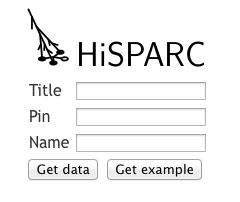
\includegraphics[scale=0.6]{jsparc_get_data}
    \caption{Het formulier waarmee zowel data van een sessie of een voorbeeld is aan te 
   		vragen.}
    \label{fig:get_data}
\end{figure}

In \figref{fig:get_data} is te zien dat de pagina in het begin vrij leeg is, er worden alleen het \hisparc logo en een
formulier waarop je de sessie-titel, de pin-code en je naam kunt invullen 
afgebeeld. Een analyse sessie is door jou of je leraar aan te vragen met het 
`Session Request Form'
\url{http://www.hisparc.nl/en/hisparc-data/jsparc/sessie-aanvragen/}. In de opgegeven mailbox krijg je een bericht met een link om een sessie aan te maken. HiSPARC verzamelt deze verzoeken en maakt de aangevraagde sessies regelmatig aan. Het duurt dus even voordat de sessie is aangemaakt. Als de sessie is aangemaakt krijg je een mail met een titel, code en een link voor de pagina met analyse-resultaten.

Met de gegevens uit deze laatste mail kunnen de gegevens uit een sessie worden geanalyseerd via \url{https://data.hisparc.nl/media/jsparc/jsparc.html}. Nadat het formulier is op deze lege pagina is ingevuld, klik je op de *Get data* knop 
om data op te halen. Als er geen sessie is aangemaakt kun je de web applicatie 
nog steeds gebruiken door op de `Get example' knop te klikken. Je krijgt een pagina met links grafieken, in het midden een kaart en rechts een tabel.

\section{Grafieken}

De grafieken tonen het gemeten signaal van de fotomultiplier buis van iedere detector, dit wordt ook wel een 'trace' genoemd. Er is sprake van een deeltjes-lawine als meerdere detectoren nagenoeg tegelijk een deeltje meten, dit wordt ook wel een event genoemd.

\subsection{Coincidenties}

Als meerdere stations tegelijk een event meten wordt dit een co|"{i}incidentie genoemd.
De traces voor alle detectoren van alle stations die een co\"incidentie hadden
worden in bovenste grafiek getoond (figuur \ref{fig:stationtrace}). Onder deze grafiek is in de balk te zien 
welke kleur ieder station heeft.  Langs de horizontale as staat de tijd in 
nanoseconden vanaf het begin van het event. Langs de vertikale as staat de 
sterkte van het detectorsignaal. Deze signaalsterkte is een maat voor het aantal deeltjes dat 
door de detector gaat.

\begin{figure}[H]
    \centering
    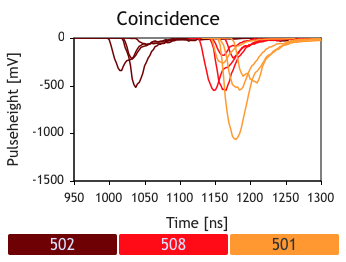
\includegraphics[scale=0.6]{jsparc_coincidence_traces}
    \caption{Traces voor alle detectoren (met dezelfde kleur) voor ieder station 
                 (verschillende kleur) tijdens co\"incidentie..}
    \label{fig:stationtrace}
\end{figure}

   Traces voor alle detectoren (met dezelfde kleur) voor ieder station 
   (verschillende kleur) tijdens coincidentie.
   
\subsection{Station grafieken}

Onder de 'Coincidence graph' kun je de traces voor ieder station afzonderlijk 
zien (figuur \ref{fig:detectortrace}). Je kunt de station selecteren door op het station nummer in de balk 
onder de coincidentie grafiek te klikken.

\begin{figure}[H]
    \centering
    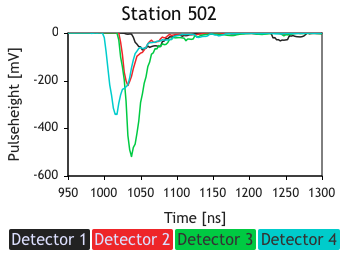
\includegraphics[scale=0.6]{jsparc_station_traces}
    \caption{Traces voor alle detectoren (verschillende kleuren) van een enkel station.}
    \label{fig:detectortrace}
\end{figure}

\subsection{Zoomen}

Je kunt op de traces in- en uitzoomen door met de cursor een gebied in de 
grafiek te selecteren (figuur \ref{fig:zoomen}). Dubbel klikken laat de hele grafiek weer zien.

\begin{figure}[H]
    \centering
    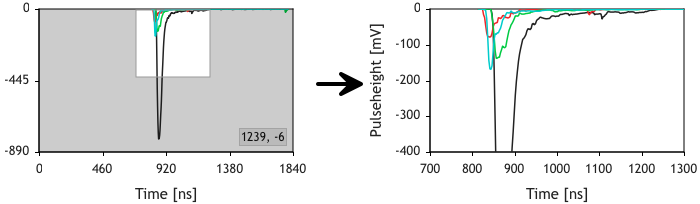
\includegraphics[scale=0.6]{jsparc_zoom_traces}
    \caption{Zoomen}
    \label{fig:zoomen}
\end{figure}

\section{Kaart}

Op de kaart naast de grafieken zijn de plaatsen van de verschillende \hisparc stations
afgebeeld (figuur \ref{fig:core}). De achtergrond wordt opgehaald bij OpenStreetMap. De kaart kan 
worden verschoven en er is in en uit te zoomen door te scrollen.

\begin{figure}[H]
    \centering
    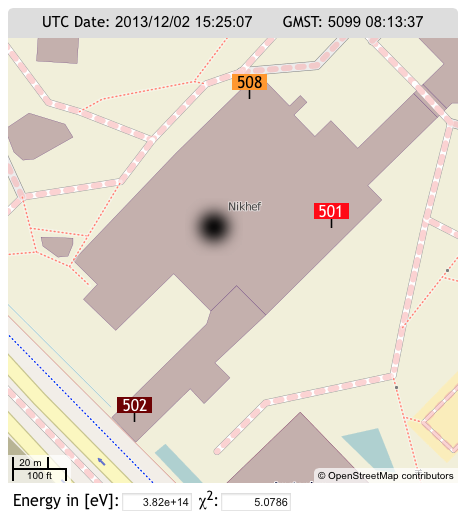
\includegraphics[scale=0.6]{jsparc_map}
    \caption{De plaatsen van de stations en het midden van de deeltjes-lawine in OpenStreetMap.}
    \label{fig:core}
\end{figure}

\subsection{De positie van het midden van de deeltjes-lawine}

Midden op de kaart is een zwarte vlek te zien, deze stelt het midden van de 
deeltjes-lawine voor. Het doel van de analyse is om de plaats van het midden 
van de deeltjes-lawine te bepalen. Het aantal deeltjes per detector wordt 
hiermee zo goed mogelijk verklaard. Het midden kan over de kaart worden 
versleept. De getallen in de tabel aan de rechterkant en onder de kaart worden 
interactief aangepast. Onder de kaart is bijvoorbeeld de $chi^{2}$-waarde\footnote{De $chi^{2}$-waarde is een maat voor de fit van de gemeten en de verwachtte waarden.} 
te zien. Als het midden op de juiste plaats ligt, is deze waarde zo laag 
mogelijk.


\section{Data tabellen}

Rechts op het scherm zie je een tabel, ieder station heeft hier een eigen kolom 
(figuur \ref{fig:detectordata}).
Op de bovenste regel kun je op ieder moment de afstand van de stations tot 
het midden van de deeltjes-lawine zien. Daaronder staat een blok waarin het 
verwachtte aantal deeltjes per detector te zien is. Dit aantal wordt aan de 
hand van de signaalsterkte geschat. Het gemiddelde per station maakt deze 
waarden nauwkeuriger. Hieronder is het aantal detectoren in te stellen. Als je 
dit aantal wilt wijzigen is het verstandig om eerst de werking van het station 
te controleren. Dit kan door op het station-nummer bovenin de kolom te klikken. 
Een nieuwe pagina met de gegevens van het station voor die dag wordt in een 
nieuw tabblad getoond. Als de krommen van de detectoren op elkaar liggen, 
functioneren alle detectoren.
Op de onderste regels zijn het gemeten (Data) en het met het midden van de 
deeltjes-lawine berekende signaal (Calc.) afgebeeld. In het ideale geval zijn 
deze waarden (nagenoeg) gelijk. 
Hoe minder deze waarden van elkaar afwijken hoe kleiner chi-kwadraat wordt.

In dit geval is te zien dat de gemeten waarde voor station 501 lager is dan de verwachtte waarde. Bij station 508 is dit net andersom. We moeten de kern van de deeltjes-lawine dus van station 501 en naar station 508 bewegen. Naar linksboven of richting Noord-West.

\begin{figure}[ht]
    \centering
    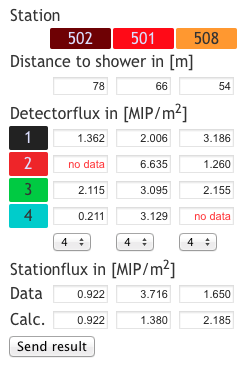
\includegraphics[scale=0.8]{jsparc_flux}
    \caption{Overzicht  van de detector data. }
    \label{fig:detectordata}
\end{figure}

\section{Submit results / Verzend het resultaat}

Nadat je de data zo goed mogelijk hebt geanalyseerd, kun je deze verzenden 
door op knop *Send results* onder de tabel te klikken. Bij de verwerking van 
de aanvraag van een sessie wordt naast een sessie-naam en pincode ook een 
uitslagen-link gestuurd. Hier is een overzicht te zien met resultaten van 
iedereen die analyses met de data van deze sessie heeft gedaan. 
   
\end{document}